% !TEX root = ./main.tex

\section{Experimental results}
\label{sec:experiment}

We now present experiments assessing the viability of our structured prediction approach
for the concrete sequential recommendation task of
trajectory recommendation.
We compare our methods to a number of non-structured baselines, over which we demonstrate significant improvements.


%
\subsection{Description of datasets}
\label{sec:dataset}

% experiment protocol: Nested cross-validation with Monte-Carlo cross-validation for the inner loop
We assess the recommendation performance %methods developed in Section~\ref{sec:trajrec}
of various methods
on trajectories extracted from Flickr photos
for the cities of Glasgow and Osaka~\cite{thomee2016yfcc100m}.
Each dataset comprises a
list of trajectories, being a sequence of points of interest (POI), as visited by various Flickr users.
The statistics of datasets are shown in Table~\ref{tab:data}.
\TODO{these seem to include a lot of irrelevant stats}
From this data, we consider the recommendation problem as posed in \S\ref{sec:trajrec}:
given a query comprising start POI and a desired trip length, can we recommend a trajectory of POIs that a visitor will enjoy?

A characteristic of these datasets is that many queries are associated with multiple trajectories, or ground truths.
The histograms of the number of ground truths for queries are shown in Figure~\ref{fig:hist}.
\TODO{only need two datasets}

% dataset stats
\begin{table}[t]
\caption{Statistics of trajectory dataset}
\label{tab:data}
\centering
\setlength{\tabcolsep}{4pt} % tweak the space between columns
\small
\begin{tabular}{l*{5}{r}} \hline
\textbf{Dataset} & \textbf{\#Photos} & \textbf{\#Visits} & \textbf{\#Traj.} & \textbf{\#Users} & \textbf{\#Queries} \\ \hline
%Edinburgh & 82,060 & 33,944 & 5,028 & 1,454 & 147 \\
Glasgow & 29,019 & 11,434 & 2,227 & 601 & 64 \\
%Melbourne & 94,142 & 23,995 & 5,106 & 1,000 & 280 \\
Osaka & 392,420 & 7,747 & 1,115 & 450 & 47 \\
%Toronto & 157,505 & 39,419 & 6,057 & 1,395 & 99 \\
\hline
\end{tabular}
\end{table}


% histogram of #ground truth
\begin{figure*}[t]
	\centering
	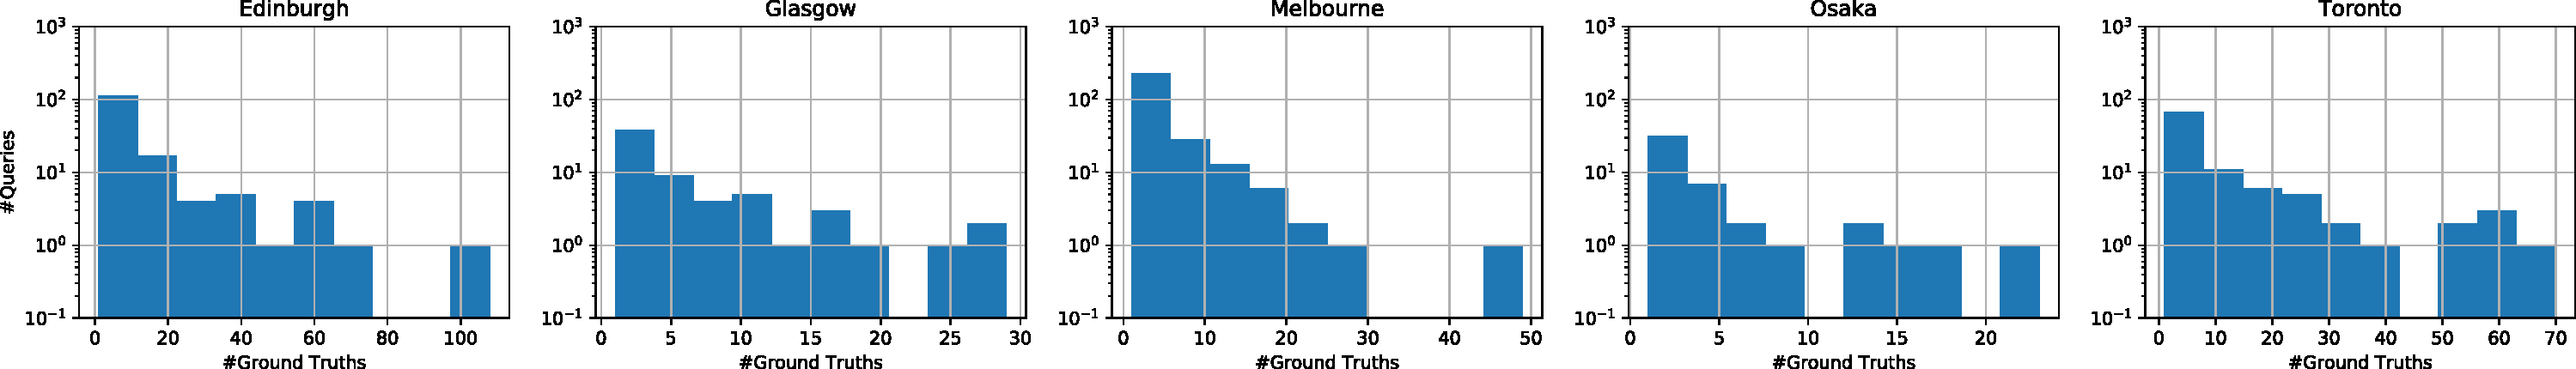
\includegraphics[width=\textwidth]{hist.pdf}
	\caption{Histogram of the number of ground truth}
	\label{fig:hist}
\end{figure*}


%
\subsection{Methods compared}

We compare the performance of our methods to three baselines.
The \textsc{Random} baseline simply keep recommending a POI sampled uniformly at random from the whole set of POIs (without replacement), until we get all the specified number of POIs.
On the other hand, the stronger \textsc{Popularity} baseline considers the popularity of each POI, 
and recommend the top-$k$ most popular places.
\textsc{PoiRank}~\cite{cikm16paper} is a generalisation of \textsc{Popularity} which considers a number of POI features in addition to its popularity,
and trains a RankSVM model to learn a score for each POI.



%
\subsection{Evaluation procedure}

% leave-one-out evaluation (with query aggregation)
%As described in Section~\ref{sec:queryagg}, 
To evaluate the performance of various methods on our datasets,
we first group the trajectories according to queries that they conform to.
We then evaluate the performance of each algorithm using leave-one-out cross validation,
where in each iteration of this procedure,
one query and its associated trajectories serves as a test point, with all other trajectories for training.
(Note that without this query aggregation, there will be considerable overlap between the train and test set, and simple nearest neighbour methods will be hard to outperform.)
% model selection (Monte Carlo CV) (with query aggregation): 90/10 random split for 5 times
Furthermore, 
all relevant hyper-parameters (e.g.\ the regularisation constant $C$) are tuned using Monte Carlo cross validation~\cite{burman1989comparative} on the training set.

% evaluation metric: kendall's Tau (mention F1, pF1)
We use three performance measures to assess the test fold performance of each algorithm:
point-F$_1$ score~\cite{ijcai15},
pairs-F$_1$ score~\cite{cikm16paper},
and
Kendall's $\tau$ (version $b$)~\cite{kendall1945,agresti2010analysis}.

Kendall's $\tau$
essentially measures the fraction of pairs of POIs that are correctly ordered in the prediction and ground truth sequences,
with adjustment for ties.
In particular,
define the rank of POIs $\mathcal{P}$ in a trajectory $\mathbf{y} = (y_1,\dots,y_K)$ as
the position of the POI within the trajectory,
\begin{align*} 
r_\mathbf{y} &= (r_1,\dots,r_j,\dots,r_{|\mathcal{P}|}), \\
r_j &= \sum_{k=1}^K (| \mathcal{P} | - k + 1)  \llb p_j = y_k \rrb, ~ j = 1, \dots, | \mathcal{P} |.
\end{align*}
The Kendall's $\tau$ score is then computed on $r_\mathbf{y}$ versus $r_\mathbf{\hat{y}}$.
Unlike the F$_1$ scores on points and pairs, 
which only care about the set of correctly recommended POIs or POI pairs,
this metric taking both factors into account.

As described previously, our methods are capable of recommending not merely a single trajectory,
but rather a list of trajectories.
While one can simply take the top recommended trajectory as the prediction,
this ignores the fact that there are likely multiple plausible trajectories for any given query.
Thus, for each performance measure,
we take the maximum over all trajectories,
i.e.,
\begin{equation*}
%\tau_b^{(i)} = 
\mathrm{perf}^{(i)}( \mathbf{y}, \hat{\mathbf{y}} ) =
\max_{(\mathbf{y}, \hat{\mathbf{y}}) \in \{\mathbf{y}^{(ij)}\}_{j=1}^{N_i} \times \{\hat{\mathbf{y}}^{(ij)}\}_{j=1}^k} 
%\tau_b(r_\mathbf{y}, r_{\hat{\mathbf{y}}}),
\mathrm{perf}(\mathbf{y}, {\hat{\mathbf{y}}}),
\end{equation*}
where $\{\mathbf{y}^{(ij)}\}_{j=1}^{N_i}$ are the ground truths for query $\mathbf{x}^{(i)}$ and
$\{\hat{\mathbf{y}}^{(ij)}\}_{j=1}^k$ are the top-$k$ recommendations.



%
\subsection{Results}
\label{sec:result}

% !TEX root = ./main.tex

\begin{table*}[t]
\caption{Experimental results on trajectory recommendation datasets. The top three rows are baselines, and the bottom four are the methods proposed in this paper. Bolded entries correspond to the best performing method for each metric; italicised entries to the next best method. Higher scores are better.}
\label{tab:result}
\centering
%\setlength{\tabcolsep}{3pt} % tweak the space between columns
\small
\begin{tabular}{l|cc|cc|cc} \hline
                    & \multicolumn{2}{|c}{\textbf{Kendall's $\tau$}}
                    & \multicolumn{2}{|c}{\textbf{F$_1$ score on points}}
                    & \multicolumn{2}{|c}{\textbf{F$_1$ score on pairs}} \\ \cline{2-7}
                    & Osaka & Glasgow 
                    & Osaka & Glasgow  
                    & Osaka & Glasgow \\ \hline
\textsc{Random}     & $0.403\pm0.025$ & $0.410\pm0.032$  
                    & $0.430\pm0.021$ & $0.451\pm0.027$  
                    & $0.057\pm0.024$ & $0.136\pm0.037$ \\
\textsc{Popularity} & $0.567\pm0.034$ & $0.646\pm0.035$  
                    & $0.601\pm0.031$ & $0.681\pm0.032$  
                    & $0.277\pm0.051$ & $0.416\pm0.050$ \\
\textsc{PoiRank}    & $0.646\pm0.040$ & $0.736\pm0.030$  
                    & $0.678\pm0.037$ & $0.764\pm0.027$  
                    & $0.425\pm0.058$ & $0.550\pm0.047$ \\
\midrule
\textsc{SP}         & $0.796\pm0.037$ & $0.865\pm0.027$  
                    & $0.817\pm0.034$ & $0.878\pm0.024$  
                    & $0.665\pm0.055$ & $0.772\pm0.040$ \\
\textsc{SPpath}     & $0.794\pm0.035$ & $0.740\pm0.034$  
                    & $0.814\pm0.032$ & $0.764\pm0.030$  
                    & $0.653\pm0.054$ & $0.591\pm0.047$ \\
\textsc{SR}         & $\mathbf{0.814\pm0.034}$ & $\mathit{0.870\pm0.025}$  
                    & $\mathbf{0.832\pm0.031}$ & $\mathit{0.887\pm0.022}$ 
                    & $\mathit{0.673\pm0.053}$ & $\mathit{0.774\pm0.039}$ \\
\textsc{SRpath}     & $\mathit{0.805\pm0.036}$ & $\mathbf{0.877\pm0.025}$ 
                    & $\mathit{0.821\pm0.033}$ & $\mathbf{0.893\pm0.021}$ 
                    & $\mathbf{0.682\pm0.054}$ & $\mathbf{0.792\pm0.038}$ \\ \hline
\end{tabular}
\end{table*}


% experimental results
The performance of three baselines and four variants based on structured prediction on two datasets are shown in Table~\ref{tab:result}.
We can see from the empirical results that all variants of structured prediction achieve very good performance.
In particular, \textsc{SR} always performs better than \textsc{SP}, 
which suggests that explicitly modelling multiple ground truths helps recommendation.

Furthermore, we observed that sub-tour elimination in training improves the ordering of recommended trajectories, 
as indicated by the F$_1$ score on pairs, 
however, this advantage will not take effect if the multiple ground truths is not modelled explicitly,
which further enforces its importance.
